\section{Présentation du TP}

Ce TP portera sur la gestion d'un luminaire RGB DALI à partir d'un automate Wago. 

\subsection{Architecture du système}
Afin de disposer du réseau DALI sur la structure de commande Wago, celle-ci doit être équipée, au minimum : 

\begin{itemize}
    \item D'un module de commande Wago. 
    \begin{itemize}
        \item 750-841 sans KNX
        \item 750-849 avec KNX
    \end{itemize}
    \item D'un module DALI Wago 750-653
    \item D'un convertisseur 24VDC/18VDC Wago (288-895) pour alimenter le bus DALI
\end{itemize}

La partie pupitre est composée de : 
\begin{itemize}
    \item Quatre boutons poussoirs (blanc, rouge, vert, bleu)
    \item Un sélecteur à 3 boutons poussoirs (haut, bas, central)
    \item Un bouton d'arrêt d'urgence
    \item Trois luminaires RGB DALI
\end{itemize}

Le \textbf{sélecteur à 3 boutons} fournit les informations \textbf{ixSelDown} et \textbf{ixSelUp} et son fonctionnement est décrit dans le tableau suivant : 

\begin{minipage}{0.15\linewidth}
    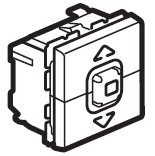
\includegraphics[width=\textwidth]{selecteur3boutons}
\end{minipage}
\begin{minipage}{0.84\linewidth}
    \begin{center}
    \begin{tabular}{|l|c|c|}
        \hline
        \textbf{Action sur le sélecteur} & \textbf{ixSelDown} & \textbf{ixSelUp} \\
        \hline
        Aucun appui & false & false \\
        \hline
        Appui sur le bouton du haut & false & true \\
        \hline
        Appui sur le bouton du bas & true & false \\
        \hline
        Appui sur le bouton central & true & true \\
        \hline
    \end{tabular} 
\end{center}   
\end{minipage}
\begin{UPSTIactivite}[2][Architecture du système][][][Préparation]
    \label{act:archi}
    \UPSTIquestion{Dessiner l'architecture matérielle faisant apparaitre les éléments Wago ainsi que les boutons poussoirs et les trois luminaires Rouge, Vert et Bleu}
    \vspace{7cm}
\end{UPSTIactivite}

D’un point de vue logiciel, on dispose de la bibliothèque \textit{DALI\_02.lib} qui offre plusieurs blocs fonctionnels
permettant d’établir les différentes commandes du bus (commande d’éclairage, de configuration, etc …) plus des
commandes étendues.



